\chapter{Simulating Limit Order Books with Generative Adversarial Networks}

With the recent development in deep learning literature owing to the development of Large Language Models and architectures such as Convolution Neural Networks (CNNs), Long-Short Term Memory (LSTM), Recurrent Neural Networks (RNNs) and Generative Adversarial Networks (GANs), a lot of recent work features the use of such models to simulate the features of the Limit Order Book.

 This chapter explores using Generative Adversarial Networks (GANs) to simulate these LOB snapshots. This chapter follows the architecture given by Cont et al. \cite{cont2023lobsimulationgan} and then conducts a simulation and ablation study on our own data. The goal is to learn the conditional probability distribution of a future LOB state given its current state. 

\section{Problem Setup}

We represent the limit order book as a collection of queue sizes around the mid-price. This is called a centered LOB snapshot. In this representation, buy queues are recorded as negative numbers. Sell queues are recorded as positive numbers. 

We model the transition of these queue sizes over a fixed time span. Price changes are naturally captured within this snapshot evolution. If the market price increases or decreases, the corresponding queues shift and change signs. A conditional model is absolutely necessary for this. The future state of the order book depends heavily on the current state. 

\section{The GAN Architecture}

A Generative Adversarial Network consists of two competing neural networks. The Generator creates synthetic LOB snapshots from a random noise seed and a state condition. The Discriminator, or Critic, evaluates whether the generated snapshot is realistic compared to real market data. 
\begin{figure}[h]
    \centering
    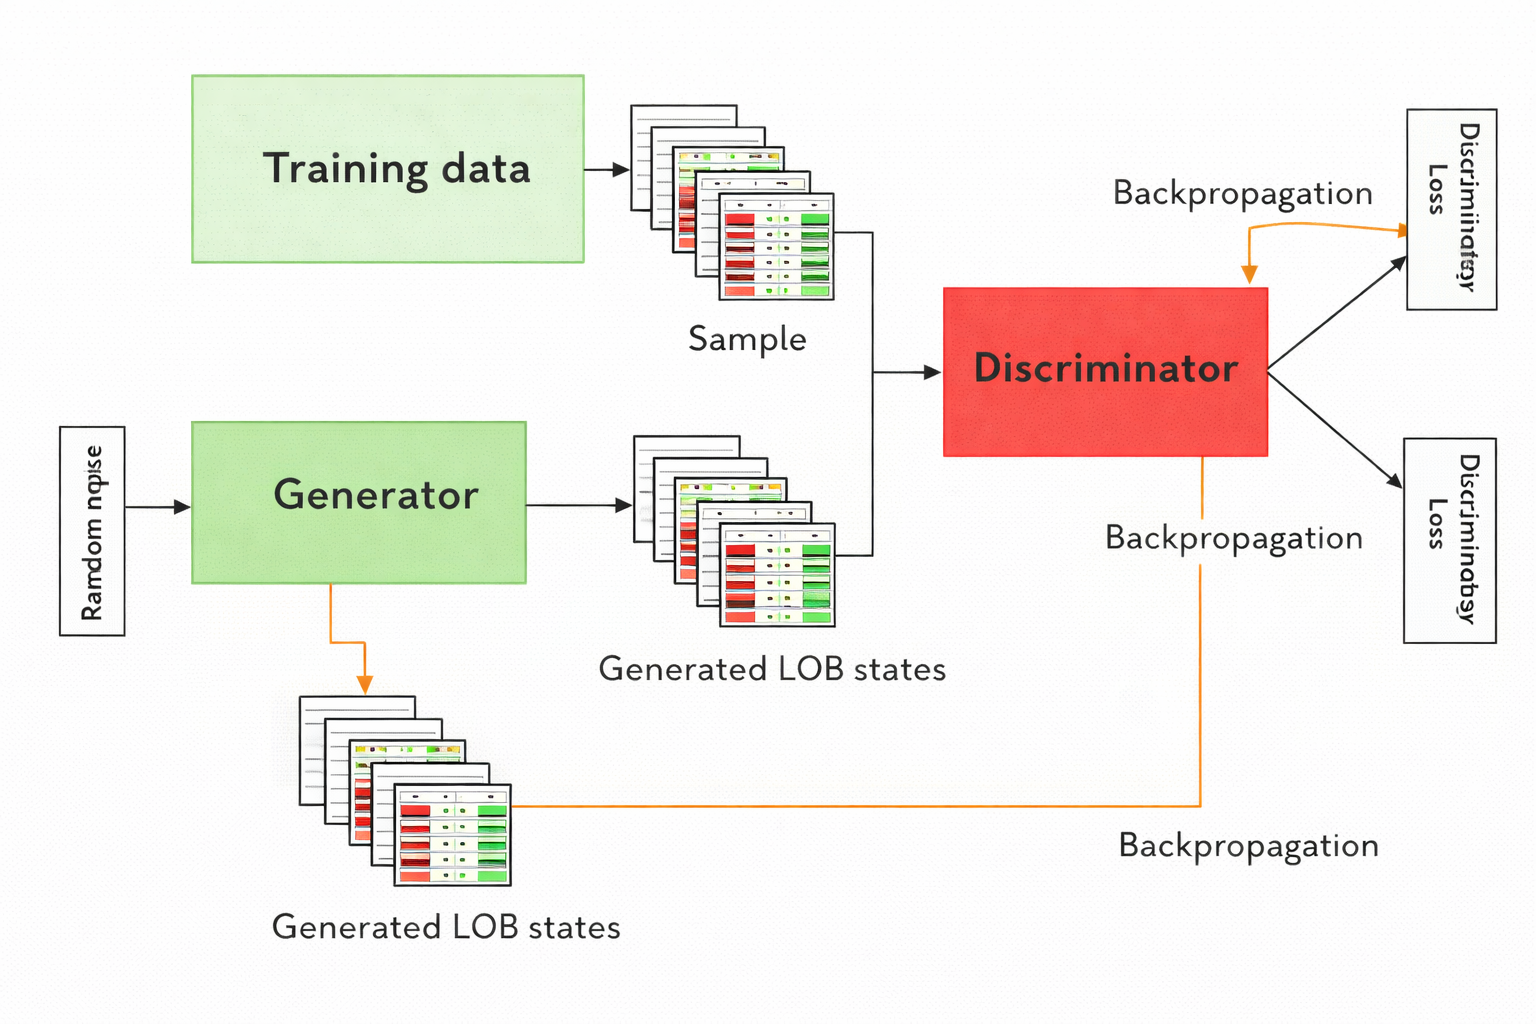
\includegraphics[width=0.82\linewidth]{GAN Architecture.png}
    \caption{\textit{Overview of the GAN Architecture}}
    \label{fig:ganarchitecture}
\end{figure}
This model utilizes a Wasserstein GAN with Gradient Penalty (WGAN-GP). Gradient clipping is applied to the critic to stabilize the training process. The model operates in a Markovian setting. This means the condition fed into the network is simply the current LOB snapshot. Both the generator and the critic use multiple fully connected layers. 
\begin{table}[h]
\centering
\begin{tabular}{ll}
\hline
Activation Hidden Layers & ReLU \\
Activation Final Layer & Linear \\
\# of hidden layers & 3 \\
Hidden Layer Size & 64 \\
$\Delta t$ & 10 seconds \\
Days of data & 1 day \\
\# Samples & $\sim 40k$ \\
Optimizer & Adam \\
Learning Rate & $1 \times 10^{-5}$ \\
Iterations & $\sim 20k$ \\
\hline
\end{tabular}
\caption{Table indicating attributes of the GAN architecture and training data used for training.}
\label{tab:gan_architecture}
\end{table}
LOB models must be symmetrical to avoid artificial arbitrage opportunities. We enforce symmetry during simulation. The model flips the LOB state with a fifty percent probability. This guarantees that unconditional price increases and decreases remain equally likely, preventing structural price drifts.

\section{Reported Results}

Cont et al. \cite{cont2023lobsimulationgan} use L3 LOB data from `lobsterdata.com`. They train their GAN on 20 days of MU Tick Data (MU is a large tick stock which rarely contains empty levels and mostly has a spread equal to the tick size) from 2016. They train their WGAN model for 300k iterations and establish some interesting results about some stylized facts.

\subsection{Marginal Density}
% \begin{figure}[h]
%     \centering
%     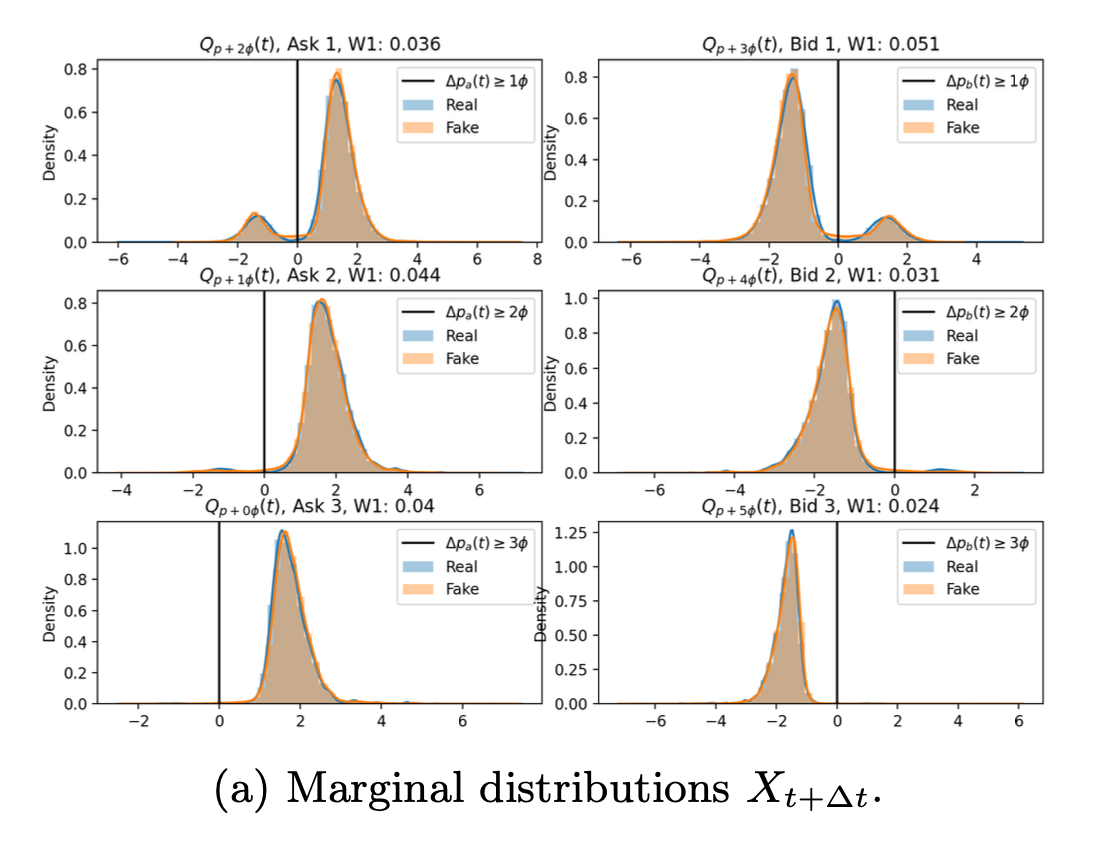
\includegraphics[width=0.82\linewidth]{GAN Marginal Density Cont.png}
%     \caption{\textit{Marginal Density as reported in Cont et al. \cite{cont2023lobsimulationgan}}}
%     \label{fig:ganmargcont}

%     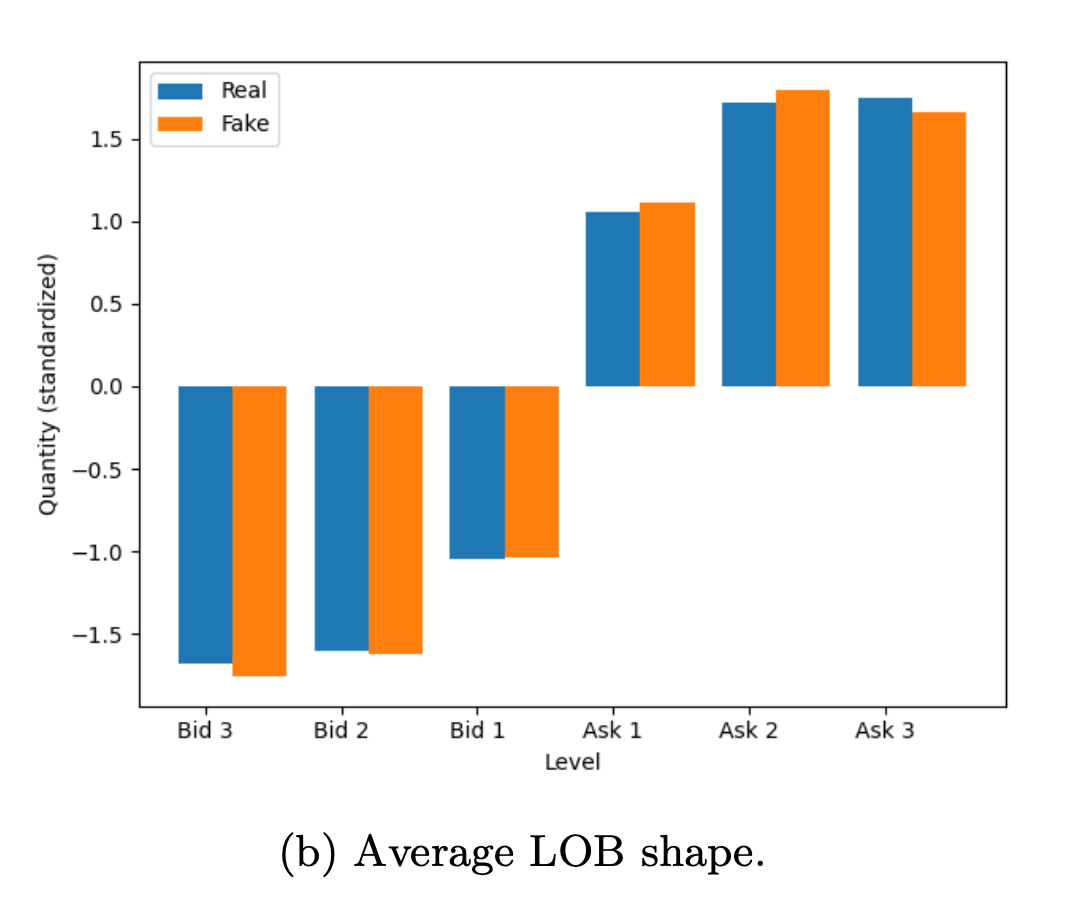
\includegraphics[width=0.82\linewidth]{GAN Average LOB Shape Cont.png}
%     \caption{\textit{Average LOB Shape as reported in Cont et al. \cite{cont2023lobsimulationgan}}}
%     \label{fig:ganavglobcont}
% \end{figure}
 Results from Cont et al.\cite{cont2023lobsimulationgan} show that the marginal distributions of $X_{t+\Delta t}$, where the overall shape of the distributions is learned well by the model. For Ask-1 and Bid-1, the negative and positive values represent samples with price changes, where the queue is depleted and becomes a queue of the opposite sign. The generated samples show slightly less probability mass in these regions compared to the real samples, which indicates fewer generated price changes. The small bumps visible in Ask-2 and Bid-2 correspond to price changes of two ticks, which have a much lower probability mass. This shows that price changes of two ticks or more are much less likely to occur.

\subsection{Average LOB Shape}
Results also show that the average limit order book shape for the real and the generated data, and both match very closely. On closer observation, the average queue sizes are slightly larger for ask quantities.

\section{Simulation and Ablation Studies}
In order to further our understanding of the topic and test the performance of the model on external data, we simulate the model mentioned in the paper on tick data of MSFT Stock (on 21st June 2012) obtained from LOBSTER. Figure 6.2 and 6.3 show the Marginal Densities obtained via our simulations. 
Our results are sub par as compared to the original paper, given the limited data and training resources, but they are still useful in establishing the validity of GANs in simulating LOBs and their properties.
\begin{figure}
    \centering
    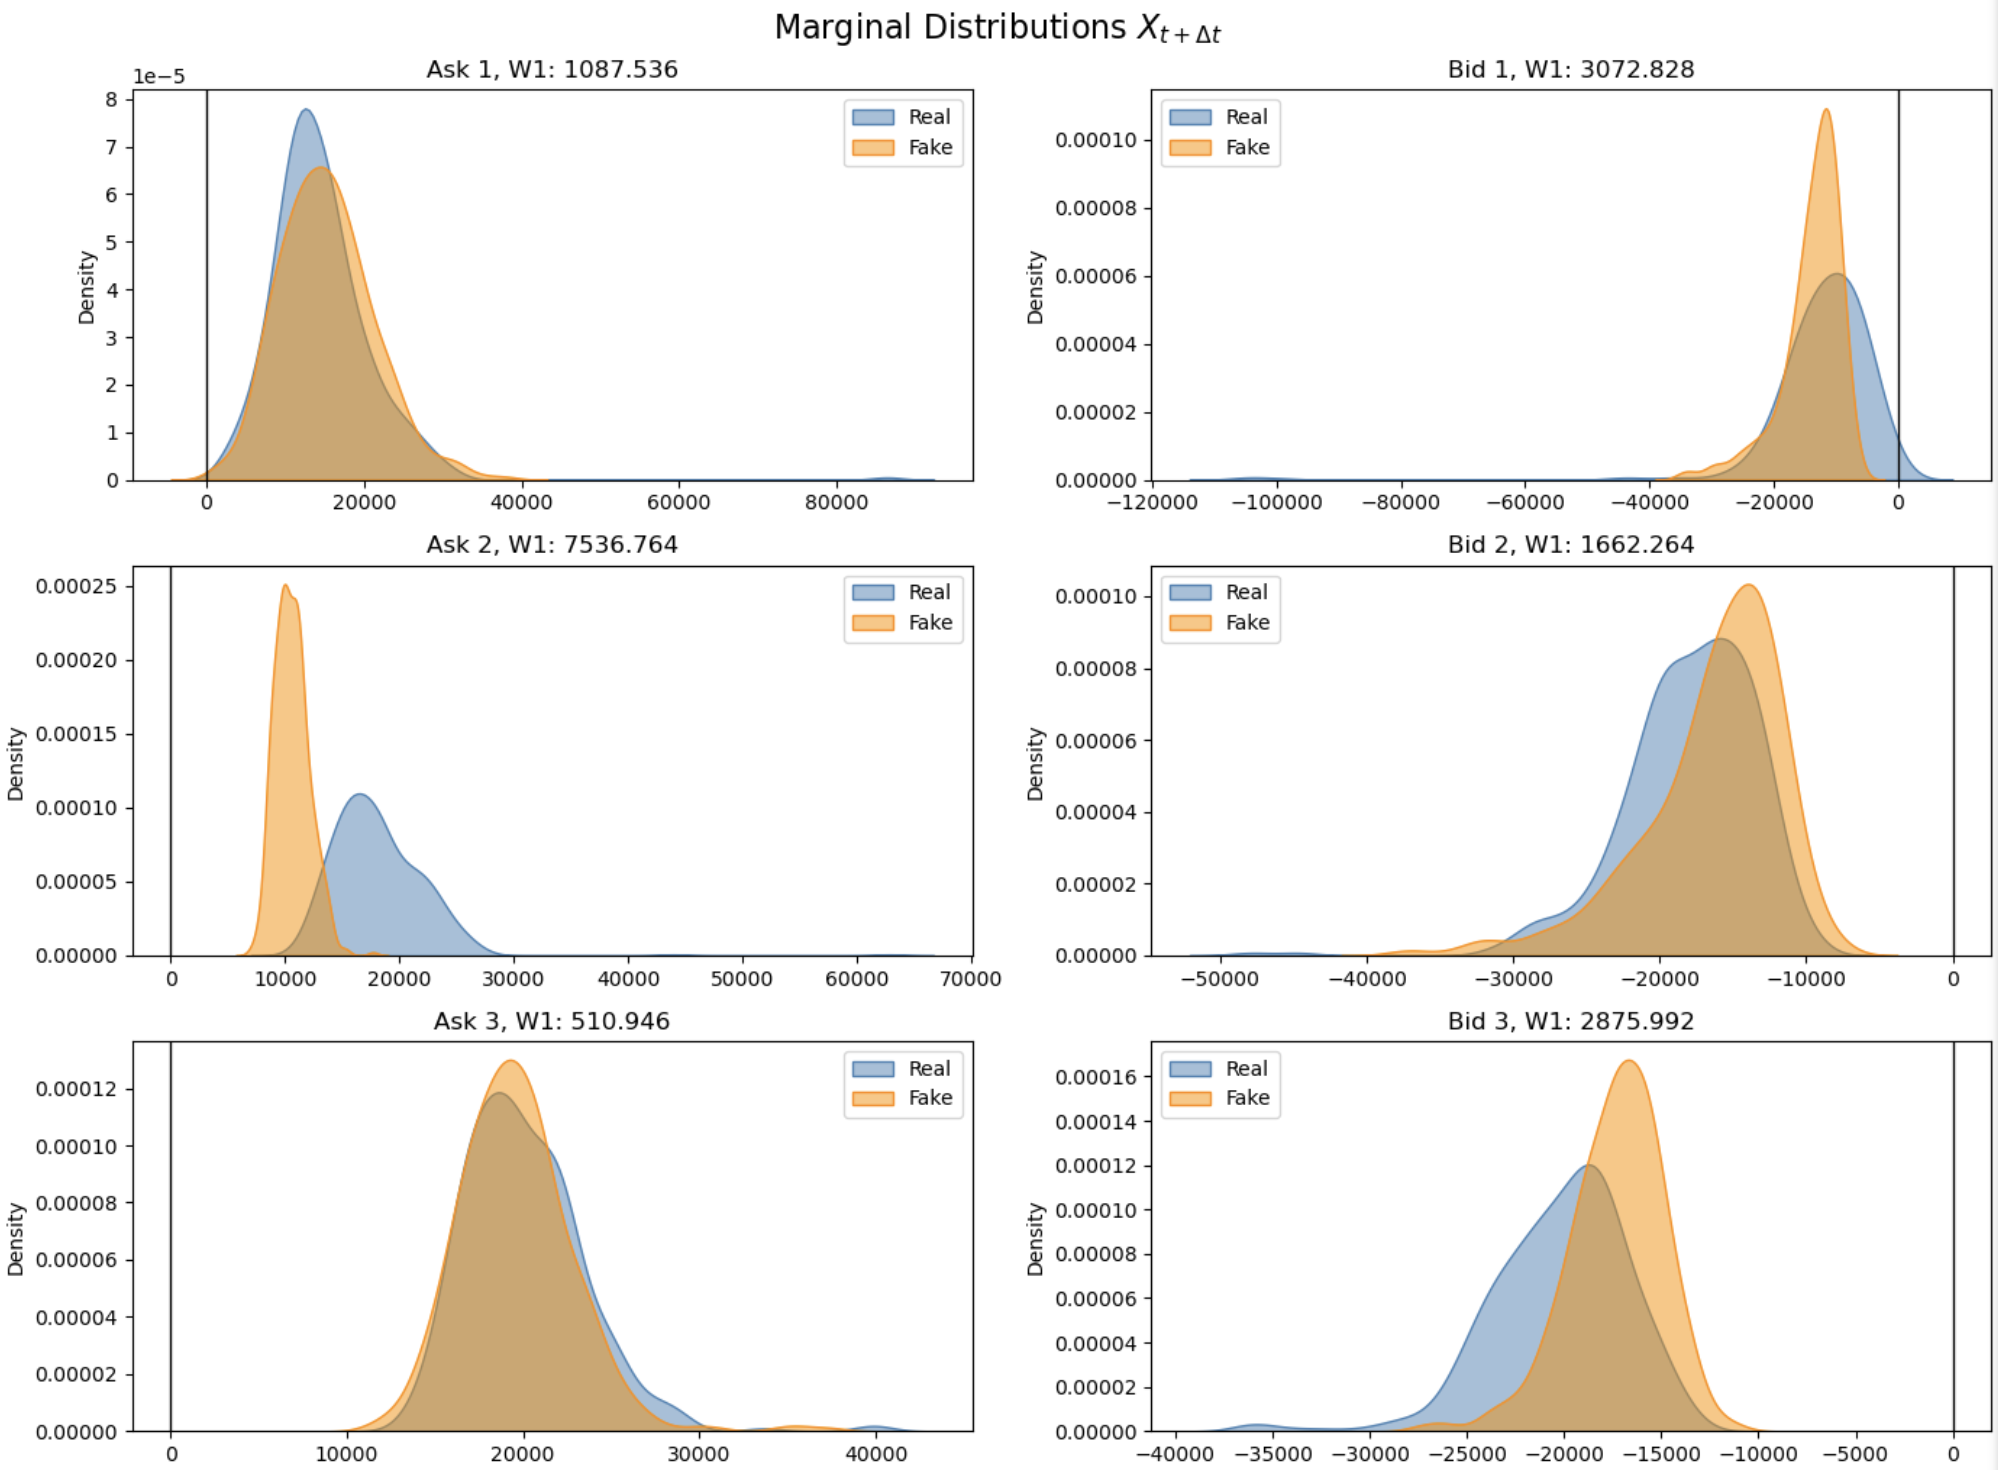
\includegraphics[width=0.82\linewidth]{GAN Marginal Densities.png}
    \caption{Marginal Densities of LOB Simulations based on MSFT Stock}
    \label{fig:ganmarg}
    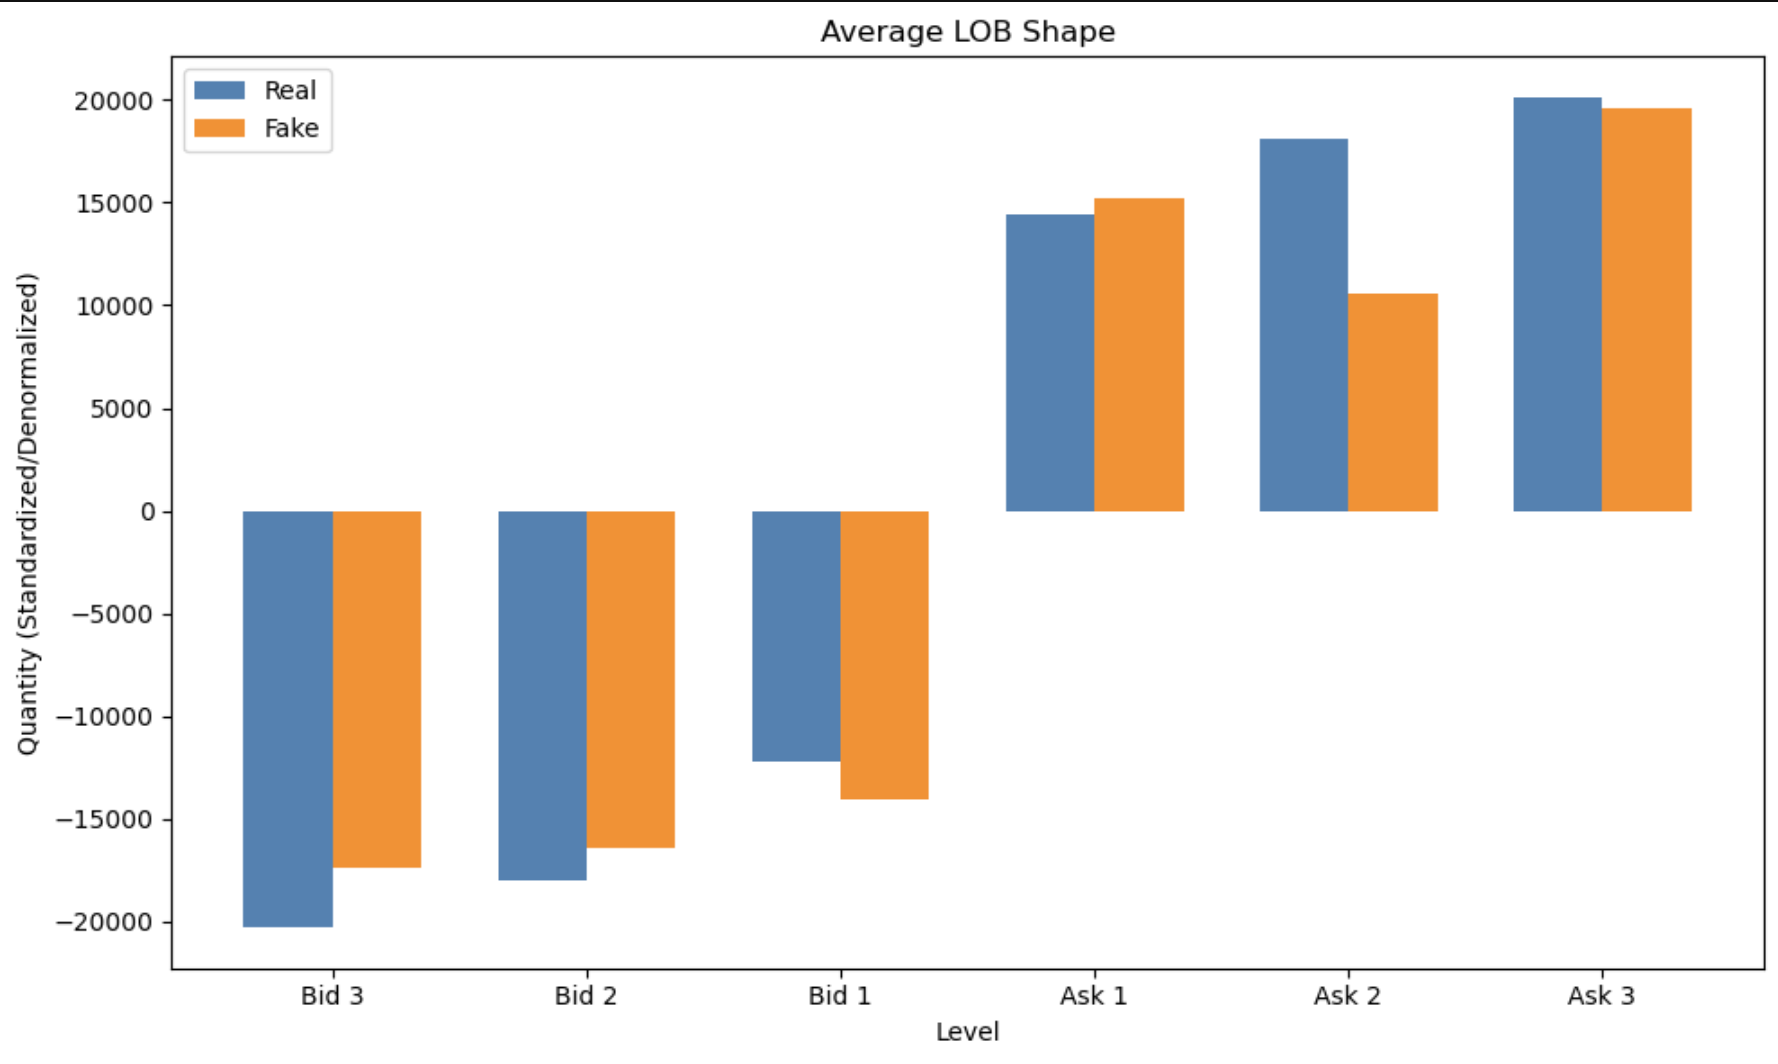
\includegraphics[width=0.82\linewidth]{GAN Average LOB Shape.png}
    \caption{Average Shape of LOB Simulations based on MSFT Stock}
    \label{fig:ganavgshape}
\end{figure}
% \section{Simulation Results}

% The trained GAN generates synthetic LOB data that closely matches empirical market data. It successfully replicates several key stylized facts:

% \begin{itemize}
%     \item \textbf{Queue Distributions:} The model accurately replicates the marginal distributions of the queue sizes.
%     \item \textbf{Order Book Shape:} The average shape of the synthetic order book matches the real order book shape perfectly. 
%     \item \textbf{Correlation Structure:} The correlation matrices of the generated order quantities are almost identical to real market data.
%     \item \textbf{Price Paths:} The generator produces realistic price paths with zero drift and appropriate volatility. 
% \end{itemize}

% The GAN significantly outperforms traditional models. For example, a benchmark Poisson order flow model produces unrealistic queue distributions and fails to generate the correct frequency of price changes.

% \subsection*{4. Interactive Market Impact}

% A useful simulator must respond realistically when a user injects trades. The GAN model organically reproduces market impact without being explicitly trained to do so. 

% \begin{itemize}
%     \item \textbf{Market Order Execution:} Executing large market orders creates a permanent price shift. This price impact strictly increases with the order size. 
%     \item \textbf{The Square-Root Law:} The relationship between order size and price impact is concave. The model successfully recovers the famous square-root law of market impact.
%     \item \textbf{Liquidity Provision:} Providing liquidity by submitting limit orders also creates a price impact. It acts as a price support. However, this impact is significantly smaller than the impact of extracting liquidity with market orders.
%     \item \textbf{Book Depth:} Placing limit orders deeper in the order book creates even less market impact than placing them at the best prices.
% \end{itemize}
\section{Conclusion}
Deep learning models are strong candidates for simulating limit order book dynamics because they can capture complex time evolution in Markov processes. Recent advances have also made training these models much easier. Many such models successfully reproduce important stylized facts and even show the concave market impact observed in real markets.

However, these models face major limitations. They are often black-box systems with low explainability, require careful hyperparameter tuning, and involve very high complexity with millions or billions of parameters. A more parsimonious and interpretable alternative is to model the transition of the order book state directly by taking the continuous-time limit and describing it through stochastic differential equations.